% \newpage
\appendix

\section{Additional Experimental Results}\label{app:additional-results}

\subsection{Evaluation on Smaller Models}
\label{app:small-model}

As presented in the \cref{tab:slm}, path-consistency substantially enhances the inference efficiency of small models on reasoning tasks. Nevertheless, due to the inherent accuracy limitations of the base models, the performance of path-consistency is inevitably influenced as well.

\begin{table*}[h]
\caption{Evaluation results of different inference techniques on Llama-3.2-1B-Instruct.}
\label{tab:slm}
\centering
\resizebox{\textwidth}{!}{
\begin{tabular}{@{}lclclcl@{}}
\toprule
                                           & \multicolumn{2}{c}{GSM8K}              & \multicolumn{2}{c}{Svamp}              & \multicolumn{2}{c}{StratrgyQA}         \\ \cmidrule(l){2-3} \cmidrule(l){4-5} \cmidrule(l){6-7}  
Method                                     & Accuracy (\%) & Tokens (\# per problem) & Accuracy (\%) & Tokens (\# per problem) & Accuracy (\%) & Tokens (\# per problem) \\ \midrule
PC                                         & 47.3          & 1430                    & 62.0          & 711                    & 63.1          & 799                    \\
AC \cite{aggarwal2023let} & 48.1          & 2748          & 61.1          & 800          & 63.9          & 1401          \\
ESC \cite{liescape}       & 47.9          & 2324          & 61.9          & 924                       & 63.7              & 1136                  \\\bottomrule
\end{tabular} 
}
\end{table*}

\subsection{Evaluation on Mistral-7B}
\label{app:mistral}
Path-consistency also generalizes to other models. Table~\ref{tab:mistral7b} reports results on Mistral-7B evaluated on GSM8K. The trend remains consistent with our main experiments: PC provides substantial efficiency gains (up to +22\% speedup and –20.3\% token reduction) while maintaining accuracy close to or slightly above the SC baseline. Notably, with a moderate confidence threshold ($C_{threshold}=0.8$), PC even improves accuracy (+0.6\%) while reducing computation by more than 11\%. These results demonstrate that path-consistency is not tied to a specific architecture and remains effective on stronger open-weight models such as Mistral-7B.
\begin{table}[h]
    % \vspace{-0.2cm}
    % \setlength{\abovecaptionskip}{0.1cm}
    \caption{Evaluation results on Mistral-7B with path-consistency on GSM8K.}
    \label{tab:mistral7b}
    \centering
    \begin{tabular}{@{}ccccc@{}}
    \toprule
    \multicolumn{1}{l}{Method} & \multicolumn{1}{l}{$C_{threshold}$} & \multicolumn{1}{l}{Accuracy (\%)} & \multicolumn{1}{l}{Speedup (\%)} & \multicolumn{1}{l}{Decrease (\%)} \\ \midrule
    SC                         & -                                   & 59.7                              & -                                & -                                \\ \midrule
    \multirow{3}{*}{PC}        & 0                                   & 58.5                              & +22.0                            & -20.3                            \\ 
                             & 0.8                                 & 60.3                              & +11.1                            & -11.4                            \\ 
                             & 0.9                                 & 60.4                              & +6.2                             & -6.6                            \\ \bottomrule
    \end{tabular}
    % \vspace{-0.2cm}
\end{table}

\subsection{Evaluation on Long-Chain Reasoning}
\label{app:long-chain}
Path-consistency is primarily designed for short-form chain-of-thought scenarios where solution paths consist of semantically discrete reasoning steps. In such tasks, path-consistency effectively reduces unnecessary token generation and accelerates inference. 

\begin{wraptable}{r}{0.5\textwidth}
% \vspace{-5mm}
  \caption{Evaluation results on AIME2025.}
  \label{tab:long chain}
% \vspace{-1mm}
\begin{scriptsize}
\setlength{\tabcolsep}{16pt}
\begin{tabular}{@{}lll@{}}
\toprule
Method            & Accuracy (\%) & Decrease (\%) \\ \midrule
Self-consistency                & 60.0          & -             \\
Path-consistency                & 76.7          & -4.1\%        \\ \bottomrule
\end{tabular}
\end{scriptsize}
\end{wraptable}%
As shown in Table \ref{tab:long chain}, to evaluate the performance on longer reasoning chains, we have added experiments on the AIME2025 dataset using DeepSeek-V3, which produces long CoT sequences. The results show that while the speedup effect remains present on long chains, it is less pronounced, achieving a 4\% reduction in token consumption. Meanwhile, there is a substantial improvement in accuracy when applying path-consistency, because path-consistency filter out early unstable reasoning branches and enforce prefix agreement, which helps long CoT sequences converge to more coherent and correct solutions.

% \subsection{Statistical Stability of Repeated Runs}
% \label{app:statistical-stability}

% Self-consistency is a sampling-based method, where each prediction is obtained by aggregating multiple sampled reasoning paths. Thus, the reported results already reflect multi-sample answer aggregation under a fixed branch budget. Running full repeated experiments over all datasets and thresholds would require substantial additional computation, so we provide repeated-run statistics on a representative setting in the Appendix. We focus on GSM8K because it is a standard arithmetic reasoning benchmark and is also used for the detailed analysis of confidence thresholds and prefix levels in the main text.

% To assess the stability of path-consistency under sampling randomness, we repeated the GSM8K experiment with Llama3-8B. The repeated runs use the same model, prompt template, decoding hyperparameters, and branch budget, with independent sampling randomness. As shown in Table~\ref{tab:gsm-stability}, path-consistency shows stable token reduction and latency speedup across repeated runs.

% \begin{table}[h]
% \centering
% \caption{Statistical stability of path-consistency on GSM8K with Llama3-8B. Results are reported as value $\pm$ standard deviation.}
% \label{tab:gsm-stability}
% \resizebox{\linewidth}{!}{
% \begin{tabular}{lcccc}
% \toprule
% Method & Accuracy (\%) & Speedup (\%) & Tokens (\# per problem) & Token Reduction (\%) \\
% \midrule
% PC ($C=0$)   & $66.6 \pm 0.28$ & $28.9 \pm 0.50$ & $73.37 \pm 0.47$ & $-24.0 \pm 0.38$ \\
% PC ($C=0.7$) & $67.1 \pm 0.38$ & $18.0 \pm 0.14$ & $81.09 \pm 0.05$ & $-16.1 \pm 0.08$ \\
% PC ($C=0.8$) & $67.8 \pm 0.19$ & $17.4 \pm 0.86$ & $80.91 \pm 0.88$ & $-16.2 \pm 0.69$ \\
% PC ($C=0.9$) & $66.6 \pm 0.10$ & $10.2 \pm 0.26$ & $87.01 \pm 0.92$ & $-9.9 \pm 0.87$ \\
% \bottomrule
% \end{tabular}
% }
% \end{table}

\section{Analysis of Prefix Selection}
\label{app:prefix-selection-analysis}

\subsection{Sensitivity to Confidence Thresholds}
\label{app:confidence-threshold}

As shown in Figure \ref{fig:confidence-threshold}, we examined the relationship between the confidence of the majority element in the tenth branch of the self-consistency baseline and the final answer across all datasets. It was observed that a confidence level around 0.8 serves as a critical threshold for determining the correctness of the final answer. Therefore, selecting confidence levels in the range of [0.7, 0.8, 0.9] is a more appropriate choice.

\subsection{Effect of High-Confidence Prefix Promotion}
\label{app:high-confidence}

As illustrated in the Figure \ref{fig:distribution}, the distribution of confidence for the final answers across all samples is shown. The implementation of path-consistency has led to a significant increase in the number of high-confidence answers, while reducing the number of samples with confidence levels around 0.5. This suggests that path-consistency effectively resolves many ambiguous cases. Consequently, this approach not only avoids compromising task accuracy but may even enhance it.

% \onecolumn
\begin{figure}[htbp]
    \begin{minipage}{0.4\textwidth}
        \centering
        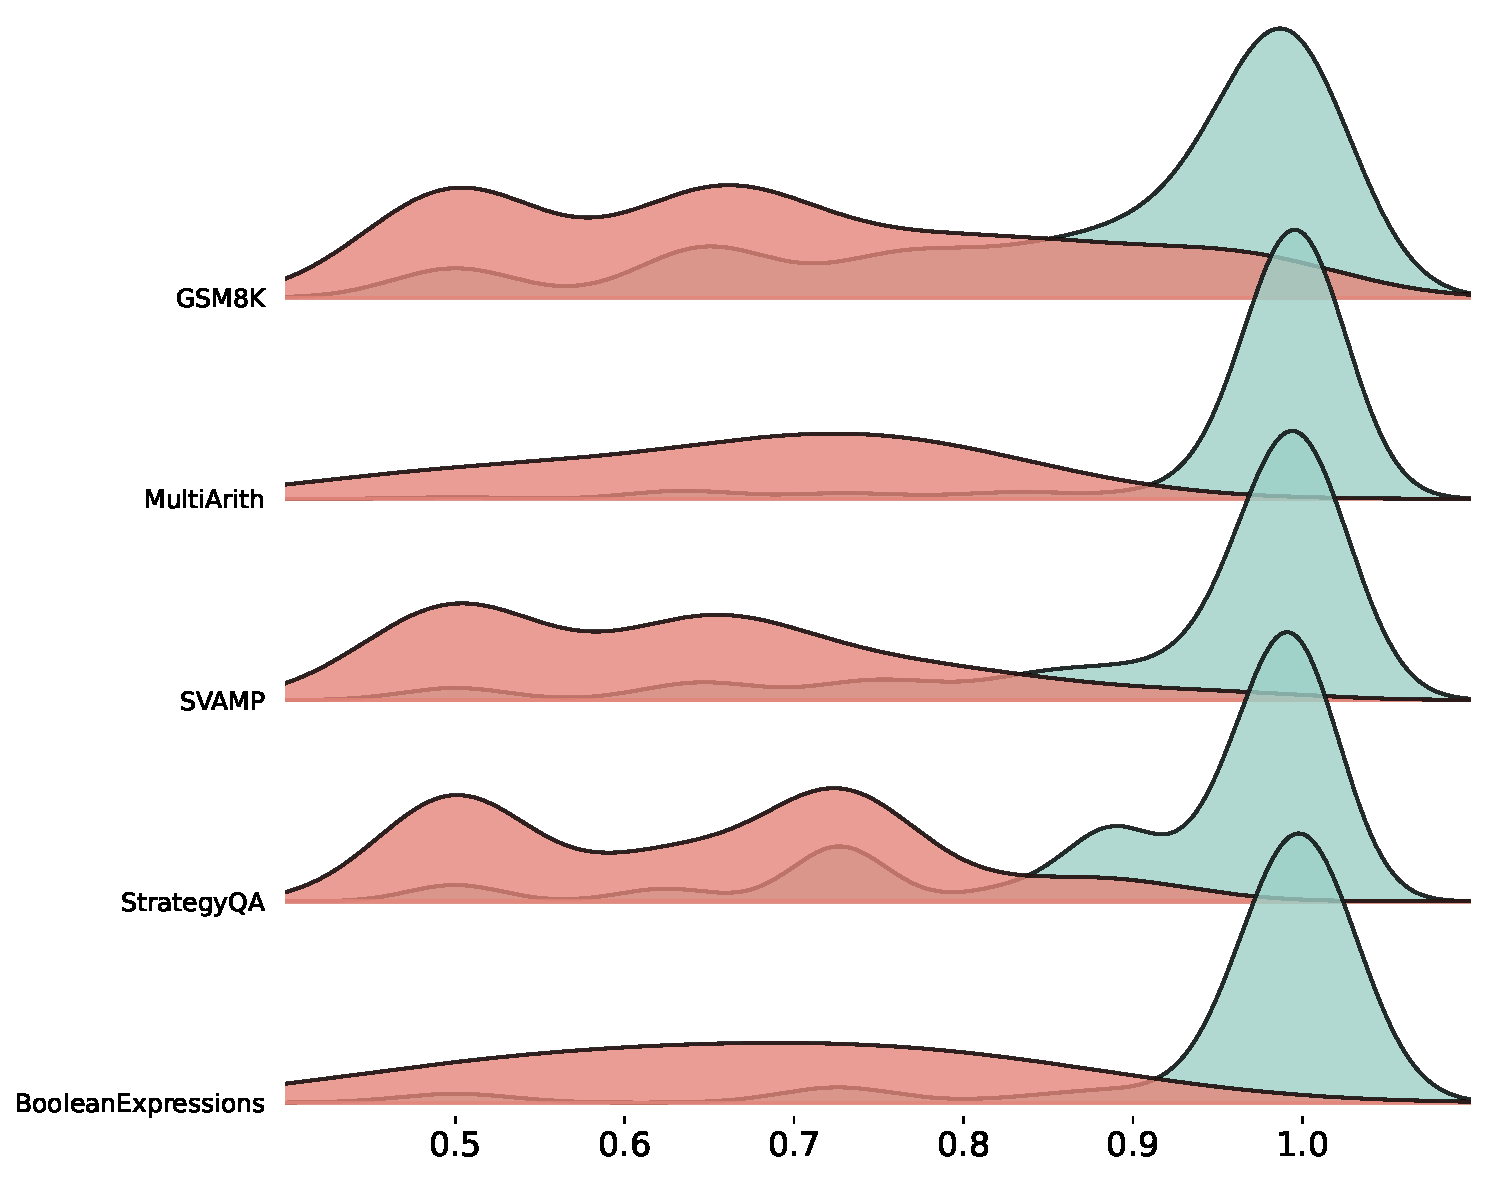
\includegraphics[width =\textwidth]{figures/conf.pdf}
        \captionof{figure}{The distribution of the majority element's confidence across all samples when self-consistency reaches the 10$^{th}$ branch.}
        \label{fig:confidence-threshold}
    \end{minipage}
    \begin{minipage}{0.55\textwidth}
        \begin{minipage}{0.49\textwidth}
            \centering
            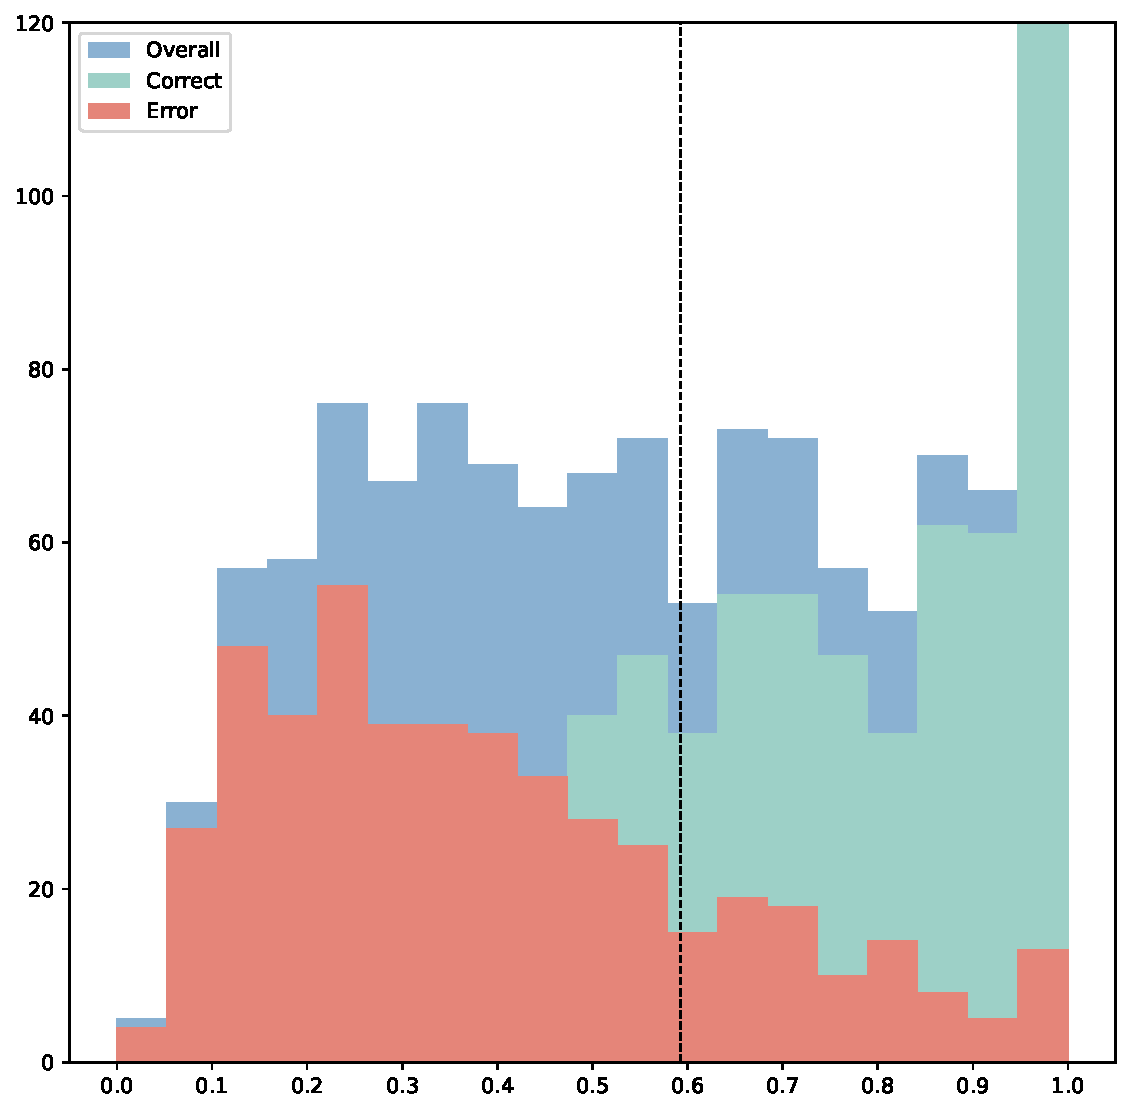
\includegraphics [width =\textwidth]{figures/base.pdf}
            \subcaption{Baseline}
            % \captionsetup{font=small}
            % \captionof{figure}{The speedup of inference by path-consistency at different prefix levels.}
            \label{fig:speedup_2}
        \end{minipage}
        \begin{minipage}{0.49\textwidth}
            \centering
            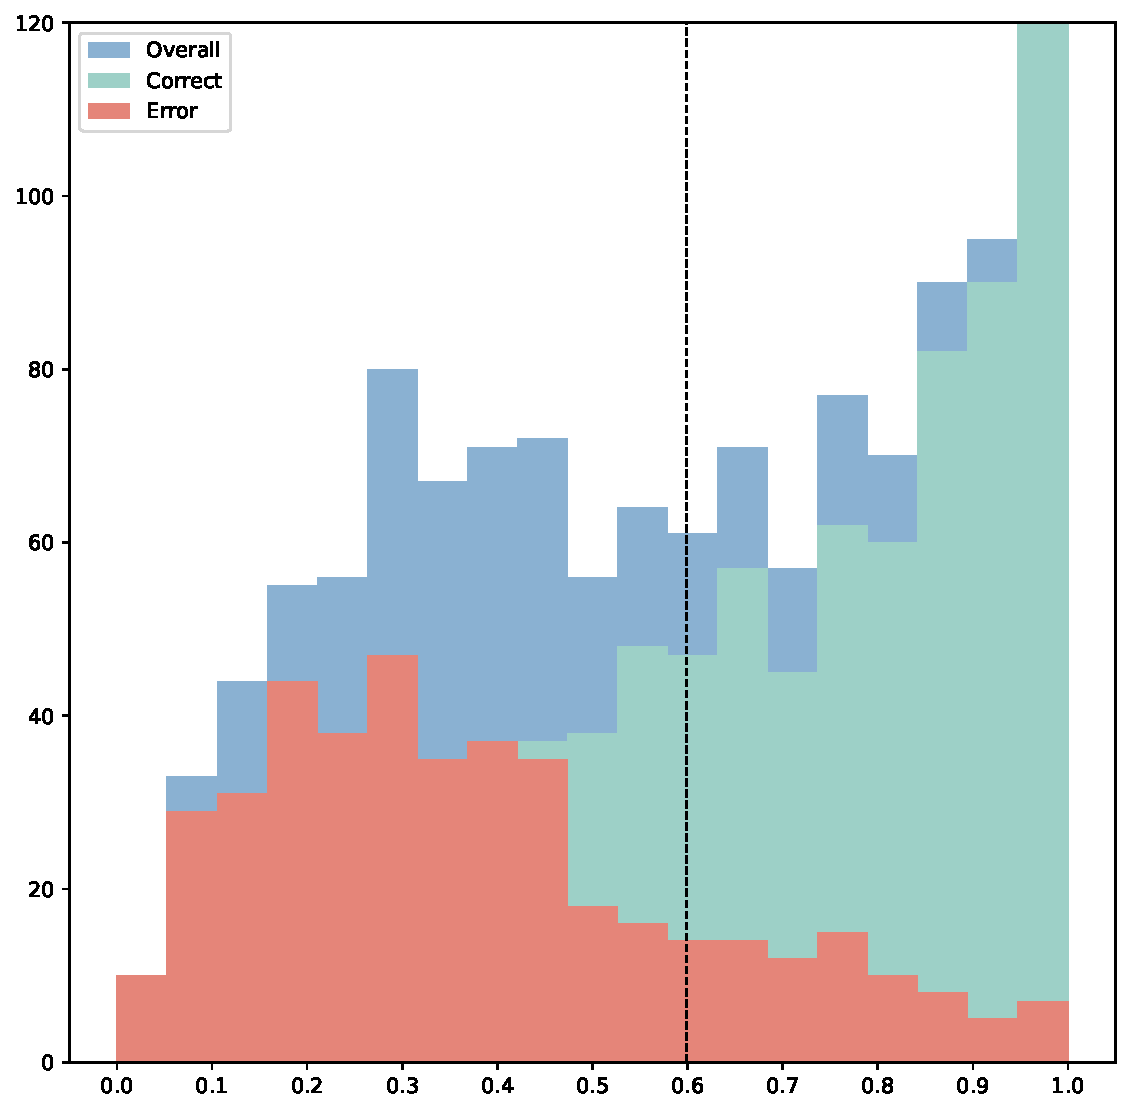
\includegraphics [width =\textwidth]{figures/c0.8.pdf}
            \subcaption{$C_{threshold}$ = 0.8}
            % \captionsetup{font=small}
            % \captionof{figure}{The decrease of token number by path-consistency at different prefix levels.}
            \label{fig:token_2}
        \end{minipage}
        \captionof{figure}{The distribution of confidence for the final answers across all samples on GSM8K.}
        \label{fig:distribution}
    \end{minipage}
\end{figure}

\subsection{Case Study on Prefix Correction}
\label{app:prefix-correction}

We analyzed the per-branch behavior of PC and found that prefix correctness does not need to be perfect in early iterations. Let's see this case:

\begin{table}[h]
    \setlength{\abovecaptionskip}{0.1cm}
    \centering
    \small
    \begin{tabularx}{0.95\columnwidth}{@{}X@{}}
        \toprule
        \textbf{Input:} \\
        \{"input":"Two girls each got 1\/6 of the 24 liters of water. Then a boy got 6 liters of water. How many liters of water were left?","target":10\} \\\\

        \textbf{Output:} \\
\{"id": 80, "result": 1, "target": 10, "answer": 10.0, \\
"answers": [8.0, 10.0, 14.0, 14.0, 14.0, 2.0, 14.0, 14.0, 10.0, 16.0, 10.0, 10.0, 10.0, 10.0, 12.0, 16.0, 14.0, 2.0, 10.0, 14.0], \\
"tokens\_gen": [70, 90, 63, 76, 84, 52, 57, 59, 54, 61, 15, 15, 15, 15, 29, 68, 65, 76, 94, 77], \\
"prefix\_level": [0, 0, 0, 0, 0, 1, 1, 1, 1, 1, 2, 2, 2, 2, 2, 0, 0, 0, 0, 0], ...\} \\
        \bottomrule
    \end{tabularx}
\end{table}

In this GSM8K instance using the Llama-3.2-1B-Instruct model, the first several sampled branches do not converge to the correct answer, and the initially extracted prefix is itself incorrect. However, as the sampling branches expands, the distribution shifts, the confidence of the current prefix falls below the Beta-gated threshold, and PC automatically discards the erroneous prefix. This “prefix correction” step allows later branches to align toward the correct reasoning (final answer: 10 liters), despite early inconsistencies.

This illustrates that iterative prefix selection does not increase the risk of propagating early minority errors. Instead, incorrect prefixes are statistically unlikely to survive multiple levels of gating: each Beta gate independently requires a majority concentration above the promotion threshold. As shown in the appendix, the probability that a wrong prefix is promoted across multiple levels decays exponentially with depth. Thus, even in cases where early reasoning is noisy or inconsistent, the PC mechanism naturally self-corrects, preventing error amplification and improving stability relative to standard SC.

\section{Computational Overhead}
\label{app:overhead}

As shown in Table \ref{tab:overhead}, we empirically evaluated the runtime cost of path-consistency on GSM8K using Llama3-8B with 20-branch sampling per problem. The additional overhead of prefix extraction and Beta confidence evaluation was negligible compared to the model sampling time. 
\begin{table}[h]
\centering
\caption{Relative Time Overhead of Beta Evaluation and Prefix Extraction}
\label{tab:overhead}
\begin{tabular}{@{}lll@{}}
\toprule
Component        & Time (s) & Ratio to Generation Time \\ \midrule
Model generation           & 2.2               & 100\%                             \\
Beta confidence evaluation & 0.000096          & 0.0044\%                          \\
Prefix extraction          & 0.00013           & 0.0059\%                          \\ \bottomrule
\end{tabular}
\end{table}

% \newpage
\section{Analysis of Beta-Gated Prefix Promotion}
\label{app:promotion-soundness}
\begin{Theorem}[Single-Level Soundness of Beta-Gated Prefix Selection]
\label{thm:single-level}
Consider a fixed level of prefix extraction with the following setup:
\begin{itemize}
    \item $\mathcal A$ denotes a finite answer set.
    \item The algorithm performs promotion checks at a sequence of increasing sample counts:
    \[
    0 < n^{(1)} < n^{(2)} < \dots < n^{(K)} = n_{\max}.
    \]
    At each check $k$, we draw the first $n^{(k)}$ i.i.d.\ samples:
    \[
    X_1, \dots, X_{n^{(k)}} \in \mathcal A.
    \]
    \item For each $a\in\mathcal A$, let $\pi(a) := \Pr(X_i = a)$ denote the model's sampling probability under the prefix. The correct answer is $a^\star$ with
    \[
    q := \pi(a^\star), \qquad R := 1-q = \sum_{a \neq a^\star} \pi(a).
    \]
    \item For each check $k$, define the observed counts:
    \[
    N_a^{(k)} := \sum_{i=1}^{n^{(k)}} \mathbf{1}\{X_i = a\},
    \qquad
    \hat a^{(k)} := \arg\max_{a\in \mathcal A} N_a^{(k)},
    \qquad
    s^{(k)} := N_{\hat a^{(k)}}^{(k)}.
    \]
\end{itemize}

Assume a Beta-gated promotion threshold $\tau \ge 0.5$, where promotion occurs at check $k$ if
\[
T(s^{(k)},n^{(k)}) := \Pr(\theta > 1/2 \mid \text{Beta}(s^{(k)}+1,\,n^{(k)}-s^{(k)}+1)) > \tau.
\]
Then, if $q \ge 1/2 + \Delta$ for some $\Delta>0$, the probability that the correct prefix fails to be promoted at check $k$ is bounded by
\[
\Pr(A_k) \le \exp\big(-2 n^{(k)} \Delta^2\big),
\]
where $A_k := \{\text{not promoted at check } k\}$.
\end{Theorem}

\begin{proof}
Promotion at check $k$ requires that $\hat a^{(k)} = a^\star$ and $T(s^{(k)},n^{(k)})>\tau$. Thus failure at check $k$ implies
\[
A_k
\subseteq
\{ N_{a^\star}^{(k)} < k_{\min}(n^{(k)},\tau) \},
\]
where
\[
k_{\min}(n,\tau) := \min\{r \in \{0,\dots,n\}: T(r,n)>\tau\}.
\]
Since $\tau\ge 0.5$, symmetry of the Beta posterior implies
\[
k_{\min}(n^{(k)},\tau) > n^{(k)}/2.
\]
Hence
\[
A_k \subseteq \{N_{a^\star}^{(k)} \le n^{(k)}/2\}.
\]
But $N_{a^\star}^{(k)}$ is a sum of $n^{(k)}$ independent Bernoulli($q$) variables with mean at least $n^{(k)}(1/2+\Delta)$. By Hoeffding's inequality,
\[
\Pr\Big(N_{a^\star}^{(k)} \le n^{(k)}/2\Big)
=
\Pr\Big(N_{a^\star}^{(k)} \le \mathbb{E}[N_{a^\star}^{(k)}] - n^{(k)}\Delta \Big)
\le
\exp\big(-2 n^{(k)} \Delta^2\big).
\]
\end{proof}

\begin{corollary}[Multi-Level Promotion Soundness]
\label{cor:multi-level}
Consider $m$ consecutive prefix-extraction levels indexed by $\ell_1,\dots,\ell_m$. At each level $\ell_j$, promotion checks occur at sample sizes $n_{\ell_j}^{(1)} < \cdots < n_{\ell_j}^{(K_j)}$, with correct-answer probabilities $q_{\ell_j} \ge 1/2 + \Delta_{\ell_j}$ and Beta thresholds $\tau_{\ell_j} \ge 0.5$. Let $A_{\ell_j}^{(k)}$ denote the failure-to-promote event at the $k$-th check of level $\ell_j$. Then, under conditional independence across levels,
\[
\Pr(\text{failure along full promotion path})
\le
\prod_{j=1}^m
\Bigg(
\sum_{k=1}^{K_j} \exp\big(-2 n_{\ell_j}^{(k)} \Delta_{\ell_j}^2\big)
\Bigg).
\]
\end{corollary}

\begin{proof}
For each level $\ell_j$, we assume the true success probability remains $q_{\ell_j} \ge 1/2 + \Delta_{\ell_j}$. This assumption is valid due to the one-time selection guarantee proved in Section~4.2, which ensures that the prefix extraction does not hurt accuracy. Thus, prefix quality is not degraded by previous selection decisions; it preserves a positive advantage $\Delta_{\ell_j}$ at every level.
At each promotion check $k$ of level $\ell_j$, requiring posterior probability
\[
\Pr(\theta_{\ell_j} > 1/2) > \tau_{\ell_j} \ge 0.5,
\]
Hoeffding’s bound implies that the probability that a truly good prefix fails to promote at this check satisfies
\[
\Pr(A_{\ell_j}^{(k)}) \le \exp(-2n_{\ell_j}^{(k)} \Delta_{\ell_j}^2).
\]
Since promotion only needs to succeed once within a level, the probability of failure across all checks of level $\ell_j$ is bounded by
\[
\Pr\Big(\bigcap_{k} A_{\ell_j}^{(k)}\Big)
\le
\sum_{k=1}^{K_j} \exp(-2n_{\ell_j}^{(k)} \Delta_{\ell_j}^2).
\]
Finally, assuming conditional independence across levels,
\[
\Pr(\text{failure along full promotion path})
=
\Pr\Big(\bigcap_{j=1}^m \bigcap_{k=1}^{K_j} A_{\ell_j}^{(k)}\Big)
\le
\prod_{j=1}^m
\Bigg(
\sum_{k=1}^{K_j} \exp(-2 n_{\ell_j}^{(k)} \Delta_{\ell_j}^2)
\Bigg).
\]

Thus the overall probability of failing to promote a prefix with true advantage $\Delta_{\ell_j}>0$ decays exponentially with the total effective sample budget across levels.
\end{proof}

\begin{corollary}[Worst-Case Wrong Answer Distribution]
\label{cor:worst-case}
For fixed total wrong-mass $R = 1-q$, the probability that a wrong answer is promoted is maximized when all wrong probability is concentrated on a single alternative. In that case, the probability of wrong promotion is
\[
\Pr(N_{a_\text{bad}} \ge k_{\min}(n,\tau)), \qquad a_\text{bad} \in \mathcal A \setminus \{a^\star\}.
\]
\end{corollary}

\begin{proof}
Let $T := \sum_{a \neq a^\star} N_a$ denote the total count of wrong answers. Then
\[
\{\exists a\neq a^\star: N_a \ge k_{\min}\} \subseteq \{T \ge k_{\min}\}.
\]
When the entire wrong-mass $R$ is assigned to a single $a_\text{bad}$, $T = N_{a_\text{bad}}$, and the inclusion becomes equality. Hence the probability of wrong promotion is maximized in this configuration.
\end{proof}


\section{Implementation Details}
\label{app:implementation}
Section \ref{sec:path-consistency} introduces the ``extract-and-sample'' process of path-consistency. Following is the code implementation of the key parts:

% Define custom colors (optional)
\definecolor{codebackground}{rgb}{0.95,0.95,0.92}
\definecolor{codeframe}{rgb}{0.8,0.8,0.8}

% Customize the appearance of the code
\lstset{
    backgroundcolor=\color{codebackground}, % Background color
    basicstyle=\ttfamily\footnotesize,      % Font style and size
    frame=single,                           % Adds a frame around the code
    rulecolor=\color{codeframe},            % Frame color
    keywordstyle=\color{blue},              % Keyword color
    commentstyle=\color{gray},              % Comment color
    stringstyle=\color{red},                % String color
    numbers=left,                           % Line numbers on the left
    numberstyle=\tiny\color{gray},          % Line number style
    stepnumber=1,                           % Number every line
    numbersep=5pt,                          % Space between line numbers and code
    tabsize=4,                              % Size of tabs
    showstringspaces=false,                 % Don't show spaces in strings
    breaklines=true,                        % Automatic line breaking
    breakatwhitespace=true,                 % Only break lines at spaces
    escapeinside={(*@}{@*)},                % Escape to LaTeX within the code
}

\subsection{Prefix Sampling}
\label{app:sample}

Randomly sample a prefix from a list of prefixes.

\begin{lstlisting}[language=Python, caption={Sample}]
def sample_prefix(prefix_list : list[str]) -> str:
    if len(prefix_list) > 0:
        prefix_index = random.randint(0, len(prefix_list)-1)
        return prefix_list[prefix_index]
    return ""
\end{lstlisting}

\subsection{Prefix Extraction}
\label{app:extract}
Generate a list of potential prefixes for future inference based on the confidence of previous answers.

\begin{lstlisting}[language=Python, caption={Extract}]
def get_prefix(answers, conf_thresh, gens, prefix, prefix_level, frq:int = 5):
    confidence = confidence_criteria(answers, conf_thresh)
    prefix_list = []
    if confidence['conf'] == False:
        return prefix, prefix_level
    for i, gen in enumerate(gens[-frq:]):
        index = len(gens) - frq + i
        parts = gen.split("answer is")
        if len(parts) > 1:
            pre_gen = parts[0]
            if answers[index] == confidence['most_common']:
                parts = re.split(r'(\.\s|\.\n|\n)', pre_gen)
                sentences = []
                for i in range(0, len(parts) - 1, 2):
                    sentences.append(parts[i] + parts[i + 1])
                sentence = ""
                for j in range(prefix_level + 1):
                    if j < len(sentences) - 1:
                        sentence += sentences[j]
                        # sentence += ". "
                prefix_list.append(sentence)
    prefix_level += 1
    return prefix_list, prefix_level
\end{lstlisting}


\subsection{Main Inference Procedure}
\label{app:inference}
A class to perform path-consistency inference using a model. It recursively samples and integrates answers based on confidence thresholds, ultimately returning a final answer.

\begin{lstlisting}[language=Python, caption={Inference}]
def inference(self, prompt: str, **kwargs):
    answers = []
    prefix_level = 0
    prefix_list = []
    reasoning = []
    times = []
    generations = []
    for branch_id in range(self.max_branch): 
        prefix = sample_prefix(prefix_list)
        prompt_plus_prefix = prompt + prefix
        start_time = time.time()
        generation = self.model.completion_function(prompt_plus_prefix,**kwargs)
        end_time = time.time()
        times.append(end_time - start_time)
        reasoning.append(prefix + generation)
        answer = extract_answer(generation, self.ans_type)
        answers.append(answer)
        generations.append(generation)
        if (branch_id + 1) % (self.max_branch / (self.max_level + 1)) == 0:
            prefix_list, prefix_level = get_prefix(answers, self.confidence_thres, reasoning, prefix_list, prefix_level)   
    final_answer = integrate_answer(answers)
    info = {'answer' : final_answer, 'answers' : answers, 'latency' : times, 'generations' : generations}
    return info
\end{lstlisting}


\subsection{Model Interface}
\label{app:model-interface}
Abstract base class for completion models defines the interface for completion models. All subclasses must implement the ``completion\_function'' method. Concrete implementation of CompletionModel using the Llama model uses a text generation model (like Llama) to generate completions based on a given prompt.

\begin{lstlisting}[language=Python, caption={Inference}]
class CompletionModel(ABC):
    @abstractmethod
    def completion_function(self, prompt: str) -> str:
        pass

class LlamaModel(CompletionModel):
    def __init__(self, generator):
        self.generator = generator

    def completion_function(self, prompt: str, **kwargs) -> str:
        prompt_list = [prompt]

        results = self.generator.text_completion(
            prompt_list,
            **kwargs
        )
        return results[-1]['generation']
\end{lstlisting}

\newpage
\section{Full Prompts}
\label{app:full-prompts}

\begin{table}[h]
    \caption{Few-shot exemplars for arithmetic reasoning.}
    \label{tab:mathprompt}
    \centering
    % \begin{tabular}{@{}l@{}}
    \begin{tabularx}{\columnwidth}{@{}X@{}}
        \toprule
        \textbf{Q:} There are 15 trees in the grove. Grove workers will plant trees in the grove today. After they are done, there will be 21 trees. How many trees did the grove workers plant today? \\
        \textbf{A:} We start with 15 trees. Later we have 21 trees. The difference must be the number of trees they planted. So, they must have planted 21 - 15 = 6 trees. The answer is 6. \\ \\
        \textbf{Q:} If there are 3 cars in the parking lot and 2 more cars arrive, how many cars are in the parking lot? \\
        \textbf{A:} There are 3 cars in the parking lot already. 2 more arrive. Now there are 3 + 2 = 5 cars. The answer is 5. \\\\
        \textbf{Q:} Leah had 32 chocolates and her sister had 42. If they ate 35, how many pieces do they have left in total? \\
        \textbf{A:} Leah had 32 chocolates and Leah’s sister had 42. That means there were originally 32 + 42 = 74 chocolates. 35 have been eaten. So in total they still have 74 - 35 = 39 chocolates. The answer is 39. \\\\
        \textbf{Q:} Jason had 20 lollipops. He gave Denny some lollipops. Now Jason has 12 lollipops. How many lollipops did Jason give to Denny? \\
        \textbf{A:} Jason had 20 lollipops. Since he only has 12 now, he must have given the rest to Denny. The number of lollipops he has given to Denny must have been 20 - 12 = 8 lollipops. The answer is 8. \\\\
        \textbf{Q:} Shawn has five toys. For Christmas, he got two toys each from his mom and dad. How many toys does he have now? \\
        \textbf{A:} He has 5 toys. He got 2 from mom, so after that he has 5 + 2 = 7 toys. Then he got 2 more from dad, so in total he has 7 + 2 = 9 toys. The answer is 9. \\\\
        \textbf{Q:} There were nine computers in the server room. Five more computers were installed each day, from monday to thursday. How many computers are now in the server room? \\
        \textbf{A:} There are 4 days from monday to thursday. 5 computers were added each day. That means in total 4 * 5 = 20 computers were added. There were 9 computers in the beginning, so now there are 9 + 20 = 29 computers. The answer is 29. \\\\
        \textbf{Q:} Michael had 58 golf balls. On tuesday, he lost 23 golf balls. On wednesday, he lost 2 more. How many golf balls did he have at the end of wednesday? \\
        \textbf{A:} Michael initially had 58 balls. He lost 23 on Tuesday, so after that he has 58 - 23 = 35 balls. On Wednesday he lost 2 more so now he has 35 - 2 = 33 balls. The answer is 33. \\\\
        \textbf{Q:} Olivia has \$23. She bought five bagels for \$3 each. How much money does she have left? \\
        \textbf{A:} She bought 5 bagels for \$3 each. This means she spent 5 * \$3 = \$15 on the bagels. She had \$23 in beginning, so now she has \$23 - \$15 = \$8. The answer is 8. \\
        \bottomrule
    \end{tabularx}
    % \end{tabular}
\end{table}

\begin{table}[H]
    \caption{Few-shot exemplars for StrategyQA.}
    \label{tab:reasoningprompt}
    \centering
    \begin{tabularx}{\columnwidth}{@{}X@{}}
        \toprule
        \textbf{Q:} Do hamsters provide food for any animals? \\
        \textbf{A:} Hamsters are prey animals. Prey are food for predators. Thus, hamsters provide food for some animals. The answer is yes. \\ \\
        
        \textbf{Q:} Yes or no: Hydrogen's atomic number squared exceeds number of Spice Girls? \\
        \textbf{A:} Hydrogen has an atomic number of 1. 1 squared is 1. There are 5 Spice Girls. Thus, Hydrogen's atomic number squared is less than 5. The answer is no. \\ \\
        
        \textbf{Q:} Yes or no: Would a pear sink in water? \\
        \textbf{A:} The density of a pear is about 0.6 g/cm\textsuperscript{3}, which is less than water. Objects less dense than water float. Thus, a pear would float. The answer is no. \\ \\
        
        \textbf{Q:} Yes or no: Is it common to see frost during some college commencements? \\
        \textbf{A:} College commencement ceremonies can happen in December, May, and June. December is in the winter, so there can be frost. Thus, there could be frost at some commencements. The answer is yes. \\ \\
        
        \textbf{Q:} Yes or no: Could a llama birth twice during War in Vietnam (1945-46)? \\
        \textbf{A:} The War in Vietnam was 6 months. The gestation period for a llama is 11 months, which is more than 6 months. Thus, a llama could not give birth twice during the War in Vietnam. The answer is no. \\ \\
        
        \textbf{Q:} Could Brooke Shields succeed at University of Pennsylvania? \\
        \textbf{A:} Brooke Shields went to Princeton University. Princeton University is about as academically rigorous as the University of Pennsylvania. Thus, Brooke Shields could also succeed at the University of Pennsylvania. The answer is yes. \\
        \bottomrule
    \end{tabularx}
\end{table}

\begin{table}[H]
    \caption{Few-shot exemplars for RuinNames.}
    \label{tab:reasoningprompt}
    \centering
    \begin{tabularx}{\columnwidth}{@{}X@{}}
        \toprule
        \textbf{Q:} Which of the following is a humorous edit of this artist or movie name: 'whitesnake'? \\
        \textbf{Options:} (A) whitesnape, (B) whitesnapke, (C) whitesnuake, (D) mwhitesnake \\
        \textbf{A:} The original name is "whitesnake". This is the name of an old English hard rock band. It is a compound word, formed by the words "white" and "snake". \\
        (A) "whitesnape": It is formed by the combination of "white" and "snake"; therefore, "snake" has been changed to "snape". Snape makes a reference to the fictional character Severus Snape in the Harry Potter series, so (A) is indeed a meaningful and funny edit. \\
        (B) "whitesnapke": It is formed by the combination of "white" and "snapke", but "snapke" is not an actual word; therefore, "whitesnapke" is not humorous. \\
        (C) "whitesnuake": It is formed by the combination of "white" and "snuake", but "snuake" is not an actual word; therefore, "whitesnuake" is not humorous. \\
        (D) "mwhitesnake": It is formed by the combination of "m", "white", and "snake", but the prefix "-m "seems arbitrary; therefore, "mwhitesnake" is not meaningful or humorous. \\
        Above the above, the only humorous edit is (A). So the answer is (A). \\\\
        
        \textbf{Q:} Which of the following is a humorous edit of this artist or movie name: 'one of our dinosaurs is missing'? \\
        \textbf{Options:} (A) ofne of our dinosaurs is missing, (B) one af our dinosaurs is missing, (C) one of our dinosaurs is pissing, (D) one of our dinosaur is missing \\
        \textbf{A:} The original name is "one of our dinosaurs is missing". This is the name of an old British movie. \\
        (A) "ofne of our dinosaurs is missing": Here "one of" is changed to "ofne", but the word "ofne" is not an actual word. \\
        (B) "one af our dinosaurs is missing": Here the word "of" is changed to "af", but the word "af" is not an actual word. \\
        (C) "one of our dinosaurs is pissing": Here the word "missing" is changed to "pissing", and "one of our dinosaurs is pissing" is indeed a very whimsical and mischievous edit. This change truly ruins the original title of the movie. \\
        (D) "one of our dinosaur is missing": Here the word "dinosaurs" is changed to "dinosaur", but "dinosaur" is singular but should be plural in the title; this change therefore feels arbitrary and not humorous. \\
        Above the above, the only humorous edit is (C). So the answer is (C). \\\\
        
        \textbf{Q:} Which of the following is a humorous edit of this artist or movie name: 'counting crows'? \\
        \textbf{Options:} (A) countingy crows, (B) counting cows, (C) courting crows, (D) coutnting crows \\
        \textbf{A:} The original name is "counting crows". This is the name of an American rock band. Historically, the band name comes from the British nursery rhyme "One for Sorrow", which is about counting of magpies. \\
        (A) "countingy crows": Here the word "counting" is changed to "countingy", but the word "countingy" is not an actual word. \\
        (B) "counting cows": Here the word "crows" is changed to "cows", and this is indeed a playful and meaningful edit that ruins the original name of the band. \\
        (C) "courting crows": Here the word "counting" is changed to "courting", and "courting" is an actual word; however, "courting crows" does not sound as humorous as "counting cows". \\
        (D) "coutnting crows": Here the word "counting" is changed to "coutnting", but the word "coutnting" is not an actual word. \\
        Above the above, the only humorous edit is (B). So the answer is (B). \\
        \bottomrule
    \end{tabularx}
\end{table}

\begin{table}[H]
    \caption{Few-shot exemplars for SalientTranslation.}
    \label{tab:errordetection}
    \centering
    \small
    \begin{tabularx}{\columnwidth}{@{}X@{}}
        \toprule
        \textbf{Q:} The following translations from German to English contain a particular error. That error will be one of the following types: Named Entities: An entity (names, places, locations, etc.) is changed to a different entity. Numerical Values: Numerical values (ordinals or cardinals), dates, and/or units are changed. Modifiers or Adjectives: The modifiers and adjectives pertaining to a noun are changed. Negation or Antonyms: Introduce or remove a negation or change comparatives to their antonyms. Facts: Trivial factual errors not pertaining to the above classes are introduced in the translations. Dropped Content: A significant clause in the translation is removed. Please identify that error. \\
        \textbf{Source:} In der Liste der Baudenkmale in Lenzen (Elbe) sind alle Baudenkmale der brandenburgischen Stadt Lenzen (Elbe) und ihrer Ortsteile aufgelistet. \\
        \textbf{Translation:} In the list of architectural monuments in Lenzen all architectural monuments of the Brandenburg city of Lenzen and its districts are listed. \\
        \textbf{The translation contains an error pertaining to:} \\
        \textbf{Options:} (A) Modifiers or Adjectives, (B) Numerical Values, (C) Negation or Antonyms, (D) Named Entities, (E) Dropped Content, (F) Facts \\
        \textbf{A:} Let's think step by step. We solve this question by first translating the source sentence to English and then by comparing our translation with the provided translation. According to Google Translate, the correct translation of the source sentence from German to English is "The list of monuments in Lenzen (Elbe) includes all the monuments in the Brandenburg town of Lenzen (Elbe) and its districts." On the other hand, the provided translation is "In the list of architectural monuments in Lenzen all architectural monuments of the Brandenburg city of Lenzen and its districts are listed." Note that Lenzen (Elbe) is changed to Lenzen in the original translation; so, there is a named entity error. Because an entity in the original source sentence is changed to a different entity in the translation, the translation contains an error pertaining to Named Entities. So the answer is (D). \\ \\
        
        \textbf{Q:} The following translations from German to English contain a particular error. That error will be one of the following types: Named Entities: An entity (names, places, locations, etc.) is changed to a different entity. Numerical Values: Numerical values (ordinals or cardinals), dates, and/or units are changed. Modifiers or Adjectives: The modifiers and adjectives pertaining to a noun are changed. Negation or Antonyms: Introduce or remove a negation or change comparatives to their antonyms. Facts: Trivial factual errors not pertaining to the above classes are introduced in the translations. Dropped Content: A significant clause in the translation is removed. Please identify that error. \\
        \textbf{Source:} Auf dieser Seite sind die Baudenkmaler der oberbayerischen Groben Kreisstadt Landsberg am Lech zusammengestellt. \\
        \textbf{Translation:} On this page are compiled the architectural monuments of the town of Landsberg am Lech. \\
        \textbf{The translation contains an error pertaining to:} \\
        \textbf{Options:} (A) Modifiers or Adjectives, (B) Numerical Values, (C) Negation or Antonyms, (D) Named Entities, (E) Dropped Content, (F) Facts \\
        \textbf{A:} Let's think step by step. We solve this question by first translating the source sentence to English and then by comparing our translation with the provided translation. According to Google Translate, the correct translation of the source sentence from German to English is "The monuments of the Upper Bavarian district town of Landsberg am Lech are compiled on this page." On the other hand, the provided translation is "On this page are compiled the architectural monuments of the town of Landsberg am Lech." Note that an important detail about the location of Landsberg am Lech is omitted in the original translation: The translation should have said "Upper Bavarian district town of Landsberg am Lech". Because a significant clause in the translation was removed, the translation contains an error pertaining to Dropped Content. So the answer is (E). \\ \\
        
        \textbf{Q:} The following translations from German to English contain a particular error. That error will be one of the following types: Named Entities: An entity (names, places, locations, etc.) is changed to a different entity. Numerical Values: Numerical values (ordinals or cardinals), dates, and/or units are changed. Modifiers or Adjectives: The modifiers and adjectives pertaining to a noun are changed. Negation or Antonyms: Introduce or remove a negation or change comparatives to their antonyms. Facts: Trivial factual errors not pertaining to the above classes are introduced in the translations. Dropped Content: A significant clause in the translation is removed. Please identify that error. \\
        \textbf{Source:} Leba ist eine Kleinstadt und ein Badeort im Powiat Leborski der polnischen Woiwodschaft Pommern. \\
        \textbf{Translation:} Eba is not a small town and seaside resort in the Powiat Leborski county of the Pomeranian Voivodeship of Poland. \\
        \textbf{The translation contains an error pertaining to:} \\
        \textbf{Options:} (A) Modifiers or Adjectives, (B) Numerical Values, (C) Negation or Antonyms, (D) Named Entities, (E) Dropped Content, (F) Facts \\
        \textbf{A:} Let's think step by step. We solve this question by first translating the source sentence to English and then by comparing our translation with the provided translation. According to Google Translate, the correct translation of the source sentence from German to English is "Łeba is a small town and seaside resort in the Powiat Leborski of the Polish Pomeranian Voivodeship." On the other hand, the provided translation is "Leba is not a small town and seaside resort in the Powiat Leborski county of the Pomeranian Voivodeship of Poland." Note that the provided sentence says, "Leba is not a small town ..." However, the translation should have been "Leba is a small town ..." Because a negation is introduced at the beginning of the sentence and has fundamentally changed the meaning of the original source, the translation contains an error pertaining to Negation or Antonyms. So the answer is (C).\\
        \bottomrule
    \end{tabularx}
\end{table}

\begin{table}[H]
    \caption{Few-shot exemplars for BooleanExpressions.}
    \label{tab:booleanexpressions}
    \centering
    \begin{tabularx}{\columnwidth}{@{}X@{}}
        \toprule
        \textbf{Q:} not ( ( not not True ) ) is \\
        \textbf{A:} Let's think step by step. \\
        Remember that (i) expressions inside brackets are always evaluated first and that (ii) the order of operations from highest priority to lowest priority is "not", "and", "or", respectively. \\
        We first simplify this expression "Z" as follows: "Z = not ( ( not not True ) ) = not ( ( A ) )" where "A = not not True". \\
        Let's evaluate A: A = not not True = not (not True) = not False = True. \\
        Plugging in A, we get: Z = not ( ( A ) ) = not ( ( True ) ) = not True = False. So the answer is False. \\ \\
        
        \textbf{Q:} True and False and not True and True is \\
        \textbf{A:} Let's think step by step. \\
        Remember that (i) expressions inside brackets are always evaluated first and that (ii) the order of operations from highest priority to lowest priority is "not", "and", "or", respectively. \\
        We first simplify this expression "Z" as follows: "Z = True and False and not True and True = A and B" where "A = True and False" and "B = not True and True". \\
        Let's evaluate A: A = True and False = False. \\
        Let's evaluate B: B = not True and True = not (True and True) = not (True) = False. \\
        Plugging in A and B, we get: Z = A and B = False and False = False. So the answer is False. \\ \\
        
        \textbf{Q:} not not ( not ( False ) ) is \\
        \textbf{A:} Let's think step by step. \\
        Remember that (i) expressions inside brackets are always evaluated first and that (ii) the order of operations from highest priority to lowest priority is "not", "and", "or", respectively. \\
        We first simplify this expression "Z" as follows: "Z = not not ( not ( False ) ) = not not ( A )" where "A = not ( False )". \\
        Let's evaluate A: A = not ( False ) = not False = True. \\
        Plugging in A, we get: Z = not not ( A ) = not not (True) = not not False = True. So the answer is True. \\
        \bottomrule
    \end{tabularx}
\end{table}


\begin{table}[H]
    \caption{Few-shot exemplars for TrackingShuffledObject.}
    \label{tab:finalpositions}
    \centering
    \begin{tabularx}{\columnwidth}{@{}X@{}}
        \toprule
        \textbf{Q:} Alice, Bob, and Claire are playing a game. At the start of the game, they are each holding a ball: Alice has a yellow ball, Bob has a blue ball, and Claire has a pink ball. As the game progresses, pairs of players trade balls. First, Claire and Alice swap balls. Then, Alice and Bob swap balls. Finally, Claire and Bob swap balls. At the end of the game, Bob has the \\
        \textbf{Options:} (A) yellow ball, (B) blue ball, (C) pink ball \\
        \textbf{A:} Let's think step by step. \\
        (0) At the start: Alice: yellow, Bob: blue, Claire: pink. \\
        (1) Claire and Alice swap balls: Alice: pink, Bob: blue, Claire: yellow. \\
        (2) Alice and Bob swap balls: Alice: blue, Bob: pink, Claire: yellow. \\
        (3) Claire and Bob swap balls: Alice: blue, Bob: yellow, Claire: pink. \\
        At the end of the game, Bob has the yellow ball. So the answer is (A). \\ \\
        
        \textbf{Q:} Alice, Bob, and Claire are playing a game. At the start of the game, they are each holding a ball: Alice has a white ball, Bob has a purple ball, and Claire has a pink ball. As the game progresses, pairs of players trade balls. First, Bob and Alice swap balls. Then, Bob and Claire swap balls. Finally, Bob and Alice swap balls. At the end of the game, Alice has the \\
        \textbf{Options:} (A) white ball, (B) purple ball, (C) pink ball \\
        \textbf{A:} Let's think step by step. \\
        (0) At the start: Alice: white, Bob: purple, Claire: pink. \\
        (1) Bob and Alice swap balls: Alice: purple, Bob: white, Claire: pink. \\
        (2) Bob and Claire swap balls: Alice: purple, Bob: pink, Claire: white. \\
        (3) Bob and Alice swap balls: Alice: pink, Bob: purple, Claire: white. \\
        At the end of the game, Alice has the pink ball. So the answer is (C). \\ \\
        
        \textbf{Q:} Alice, Bob, and Claire are dancers at a square dance. At the start of a song, they each have a partner: Alice is dancing with Lola, Bob is dancing with Rodrigo, and Claire is dancing with Patrick. Throughout the song, the dancers often trade partners. First, Alice and Bob switch partners. Then, Claire and Bob switch partners. Finally, Bob and Alice switch partners. At the end of the dance, Alice is dancing with \\
        \textbf{Options:} (A) Lola, (B) Rodrigo, (C) Patrick \\
        \textbf{A:} Let's think step by step. \\
        (0) At the start: Alice: Lola, Bob: Rodrigo, Claire: Patrick. \\
        (1) Alice and Bob switch partners: Alice: Rodrigo, Bob: Lola, Claire: Patrick. \\
        (2) Claire and Bob switch partners: Alice: Rodrigo, Bob: Patrick, Claire: Lola. \\
        (3) Bob and Alice switch partners: Alice: Patrick, Bob: Rodrigo, Claire: Lola. \\
        At the end of the dance, Alice is dancing with Patrick. So the answer is (C). \\
        \bottomrule
    \end{tabularx}
\end{table}

\begin{table}[H]
    \caption{Few-shot exemplars for LogicalDeduction.}
    \label{tab:logicaldeduction}
    \centering
    \begin{tabularx}{\columnwidth}{@{}X@{}}
        \toprule
        \textbf{Q:} The following paragraphs each describe a set of three objects arranged in a fixed order. The statements are logically consistent within each paragraph. In a golf tournament, there were three golfers: Amy, Eli, and Eve. Eve finished above Amy. Eli finished below Amy. \\
        \textbf{Options:} (A) Amy finished last, (B) Eli finished last, (C) Eve finished last \\
        \textbf{A:} Let's think step by step. \\
        (1) Eve finished above Amy: "(above) ? Eve ? Amy ? (below)". \\
        (2) Eli finished below Amy: "(above) ? Amy ? Eli ? (below)". \\
        (3) Combining (1) and (2) we get the following ordering: "(above) Eve Amy Eli (below)". \\
        According to this ordering, the person who finished last (the one at the bottom of this list) is Eli. \\
        Eli finished last. So the answer is (B). \\ \\
        
        \textbf{Q:} The following paragraphs each describe a set of three objects arranged in a fixed order. The statements are logically consistent within each paragraph. On a shelf, there are three books: a white book, a green book, and an orange book. The green book is to the right of the white book. The orange book is the rightmost. \\
        \textbf{Options:} (A) The white book is the leftmost, (B) The green book is the leftmost, (C) The orange book is the leftmost \\
        \textbf{A:} Let's think step by step. \\
        (1) The green book is to the right of the white book: "(left) ? white ? green ? (right)". \\
        (2) The orange book is the rightmost: "(left) ? white ? green orange (right)". \\
        (3) Combining (1) and (2) we get the following ordering: "(left) white green orange (right)". \\
        According to this ordering, the leftmost book is the white book. \\
        The white book is the leftmost. So the answer is (A). \\ \\
        
        \textbf{Q:} The following paragraphs each describe a set of three objects arranged in a fixed order. The statements are logically consistent within each paragraph. On a shelf, there are three books: a red book, a gray book, and a white book. The white book is to the left of the gray book. The red book is the second from the left. \\
        \textbf{Options:} (A) The red book is the leftmost, (B) The gray book is the leftmost, (C) The white book is the leftmost \\
        \textbf{A:} Let's think step by step. \\
        (1) The white book is to the left of the gray book: "(left) ? white ? gray ? (right)". \\
        (2) The red book is the second from the left: "(left) ? white red gray ? (right)". \\
        (3) Combining (1) and (2) we get the following ordering: "(left) white red gray (right)". \\
        According to this ordering, the leftmost book is the white book. \\
        The white book is the leftmost. So the answer is (C). \\
        \bottomrule
    \end{tabularx}
\end{table}

\section{Limitations and Additional Statements}
\label{app:limitations-statements}

\paragraph{Limitations.}
Path-consistency is mainly designed for short-form reasoning tasks with reusable and semantically discrete intermediate steps. For long-chain reasoning, later branches may still require substantial problem-specific generation even when a prefix is reused, making the token reduction less pronounced. In addition, the method depends on the reliability of the confidence criterion for prefix promotion. Aggressive thresholds may promote suboptimal prefixes, whereas conservative thresholds may limit token savings. Future work will explore long-chain reasoning, adaptive prefix lengths, and more robust prefix selection criteria.

\paragraph{Reproducibility.}
We provide the full prompting templates in Appendix~\ref{app:full-prompts} and the key implementation details of path-consistency in Appendix~\ref{app:implementation}. All experiments use the same maximum branch budget for self-consistency and path-consistency to ensure a fair comparison of token consumption and latency under the same multi-path reasoning setting. The main hyperparameters, including sampling temperature, top-$p$, confidence thresholds, and hardware configuration, are reported in Section~\ref{sec:evaluation}. 

\paragraph{Computational resources.}
The main experiments are conducted on a single NVIDIA GeForce RTX 3090 GPU. Path-consistency introduces only lightweight non-model operations, including confidence evaluation and prefix extraction. As shown in Appendix~\ref{app:overhead}, this overhead is negligible compared with autoregressive model generation.

\paragraph{Assets and licenses.}

This work uses publicly available datasets and open-weight language models only for research evaluation. We cite the original papers for all datasets and models used in the experiments and follow their corresponding licenses or terms of use. We do not redistribute any dataset or model weights in this work. The datasets used in the main experiments are summarized in Table~\ref{tab:dataset-licenses}.

\begin{table}[h]
\centering
\caption{Datasets used in the main experiments and their licenses or terms of use.}
\label{tab:dataset-licenses}
\resizebox{\linewidth}{!}{
\begin{tabular}{lll}
\toprule
Dataset & Source / benchmark family & License or terms of use \\
\midrule
GSM8K & Arithmetic reasoning & MIT License \\
SVAMP & Arithmetic reasoning & MIT License for the public Hugging Face version \\
ASDiv & Arithmetic reasoning & CC BY-NC 4.0 for the public Hugging Face version \\
MultiArith & Arithmetic reasoning & Apache 2.0 for the public Kaggle version \\
StrategyQA & Commonsense reasoning & MIT License for the public Hugging Face version \\
Ruin Names & BIG-Bench / BIG-Bench Hard & Apache 2.0 \\
Salient Translation & BIG-Bench / BIG-Bench Hard & Apache 2.0 \\
Boolean Expressions & BIG-Bench / BIG-Bench Hard & Apache 2.0 \\
Tracking Shuffled Objects & BIG-Bench / BIG-Bench Hard & Apache 2.0 \\
Logical Deduction & BIG-Bench / BIG-Bench Hard & Apache 2.0 \\
\bottomrule
\end{tabular}
}
\end{table}

The additional long-chain reasoning experiment in the Appendix uses AIME2025 only for evaluation. We use the publicly available evaluation set and follow its corresponding terms of use.

\paragraph{Broader impacts.}
Path-consistency aims to reduce the test-time cost of sampling-based LLM reasoning. Its positive impact is improving the efficiency and accessibility of multi-path reasoning methods by reducing token consumption and inference latency. However, as with other methods that improve LLM reasoning efficiency, the approach could also reduce the cost of unintended or harmful uses of language models. The method does not introduce new data collection, human-subject experiments, or model training, and its risks are mainly inherited from the underlying language models and benchmarks.

\paragraph{LLM usage.}
The core method, experiments, and analysis in this paper involve LLMs as the evaluated models. LLMs are used as inference backbones for generating reasoning paths under self-consistency and path-consistency. No LLM-generated data is used to train a new model in this work.

